\documentclass{beamer}

\mode<presentation>
{
  % Adjust theme. Browse themes from
  % /usr/share/texmf/tex/latex/beamer/themes/
  \useinnertheme[shadow=true]{rounded} % default from Warsaw theme
%  \useoutertheme{shadow} % default from Warsaw theme
  \useoutertheme{split}

  \usecolortheme{orchid} % default from Warsaw theme
  \usecolortheme{whale} % default from Warsaw theme
  \usecolortheme{beaver} % this overrides both orchid and whale, as far as I see, but keep them for safety

  % these override \usecolortheme above
  \setbeamercolor{frametitle}{bg=,fg=darkred!80!black}
  \setbeamercolor{frametitle right}{bg=}

  \usefonttheme[onlylarge]{structurebold}
  \setbeamerfont{block title}{size={}} % default from Warsaw theme
  \setbeamerfont{frametitle}{series=\bfseries} % probably taken care of by structurebold anyway, but keep in case useful for the future
  %% \setbeamerfont{author}{series=\bfseries}
  %% \setbeamerfont*{institute}{size=\scriptsize,series=\bfseries}
  %% \setbeamerfont{date}{series=\bfseries}

  \setbeamercovered{transparent}

  % Some fun with backgrounds:
  % \setbeamercolor{normal text}{bg=}
  % \setbeamercolor{background canvas}{bg=}
  % \setbeamertemplate{background canvas}[vertical shading][bottom=black,top=black,middle=blue!50!black]
}

\usepackage[english]{babel}
% or whatever

\usepackage[latin1]{inputenc}
% or whatever

\usepackage{times}
\usepackage[T1]{fontenc}
% Or whatever. Note that the encoding and the font should match. If T1
% does not look nice, try deleting the line with the fontenc.


\title{Shadow Maps and Projective Texturing In~X3D}

\author[Michalis Kamburelis]{Michalis Kamburelis \\ \texttt{michalis.kambi@gmail.com}}
\institute{Institute of Computer Science\\ University of Wroc{\l}aw, Poland}
\date{Web3D 2010}

% If you have a file called "university-logo-filename.xxx", where xxx
% is a graphic format that can be processed by latex or pdflatex,
% resp., then you can add a logo as follows:

\pgfdeclareimage[height=2cm]{ii-and-kambivrml}{ii-and-kambivrml}
\logo{\pgfuseimage{ii-and-kambivrml}}

\AtBeginSection[]
{
  \begin{frame}<beamer>{Outline}
    \tableofcontents[currentsection,currentsubsection]
  \end{frame}
}

\newcommand*{\codeem}[1]{\textbf{#1}}

\begin{document}

{
  % Use background on title slide only,
  % trick from http://www.tug.org/pipermail/texhax/2007-March/008035.html
  \usebackgroundtemplate{
\includegraphics[width=\paperwidth]{bg-lighter}}
  \begin{frame}
    \titlepage
  \end{frame}
}

\begin{frame}{Outline}
  \tableofcontents
  % You might wish to add the option [pausesections]
\end{frame}

\section{Motivation and Previous Work}

\subsection{Motivation}

\begin{frame}{We Want The Scenes To Look Pretty}
  \begin{columns}[T]
    \begin{column}{1in}
      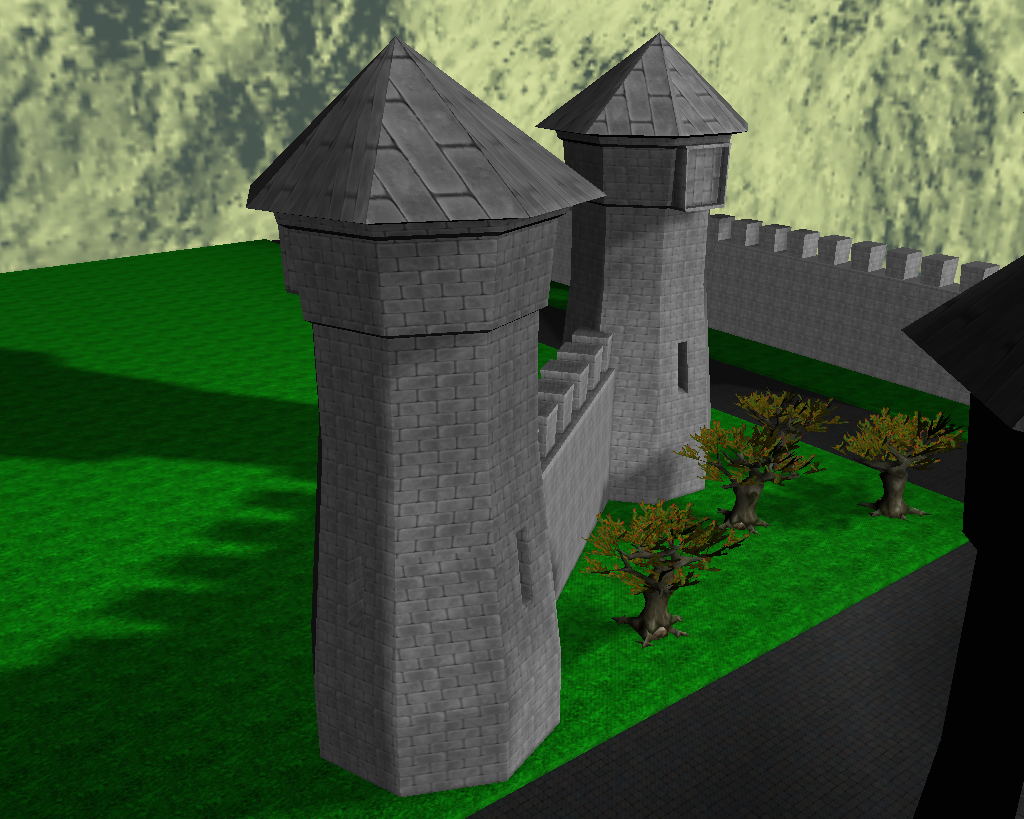
\includegraphics[width=1.5in]{../sunny_street_above_view}
    \end{column}
    \begin{column}{2.5in}
      \begin{itemize}
        \item Shadows make the scene look realistic.
        \item Shadows automatically make the impression that
          ,,more stuff is happening'' on the screen.\\
          This is even more true for dynamic scenes,
          where shadows also change dynamically.
%          So~your scenes feel even more alive.
      \end{itemize}
    \end{column}
  \end{columns}

  %% \begin{figure}
  %%   \centering
  %%   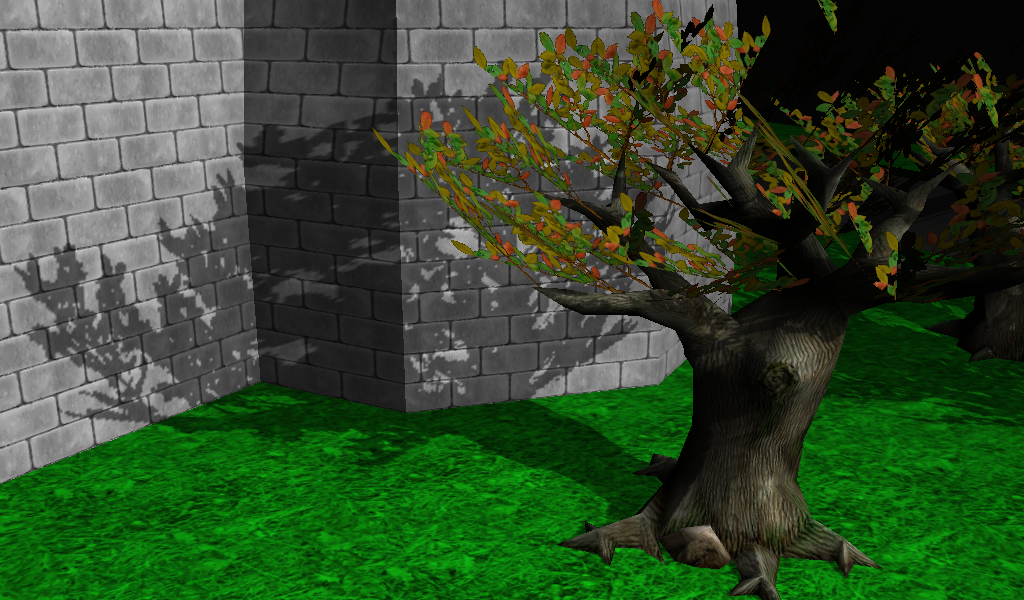
\includegraphics[width=3in]{../sunny_street_tree_hard.png}
  %% \end{figure}
\end{frame}

\begin{frame}{We Want The User To Understand What Is Displayed}
  Shadows help the mind to determine the positions of the 3D objects.\\
  Is this spider hovering or standing on the ground?

  \begin{figure}
    \centering
    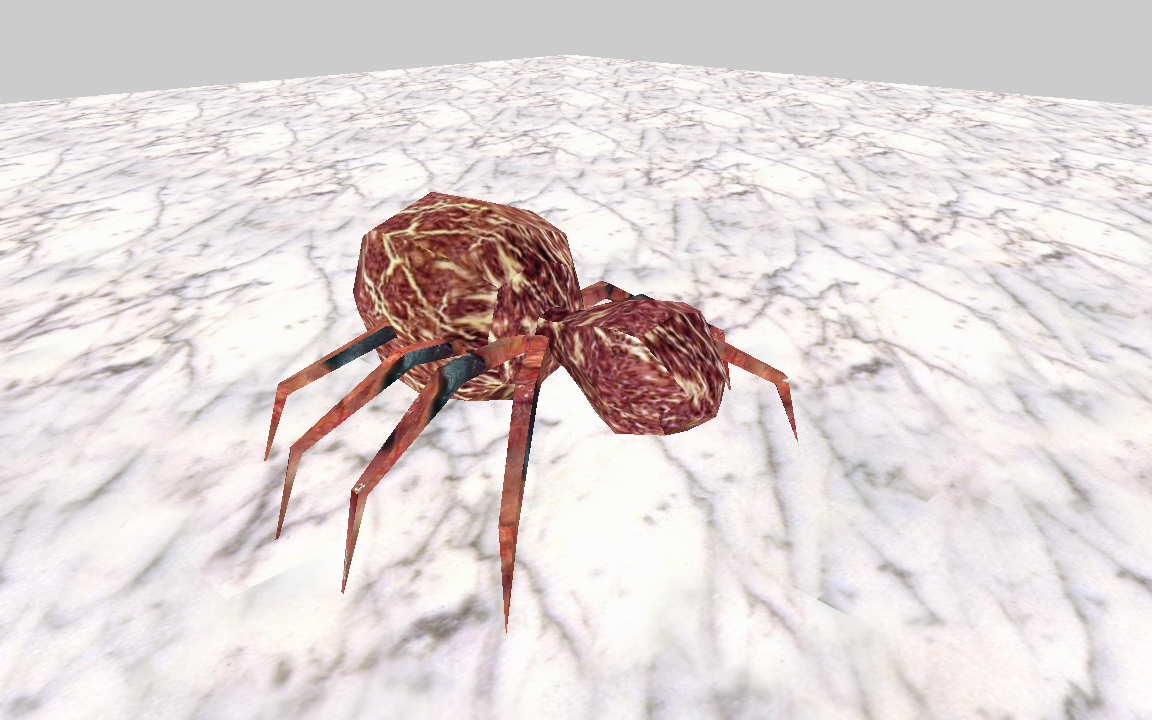
\includegraphics[width=1.8in]{spider_shadow_no}
    \hskip10pt
    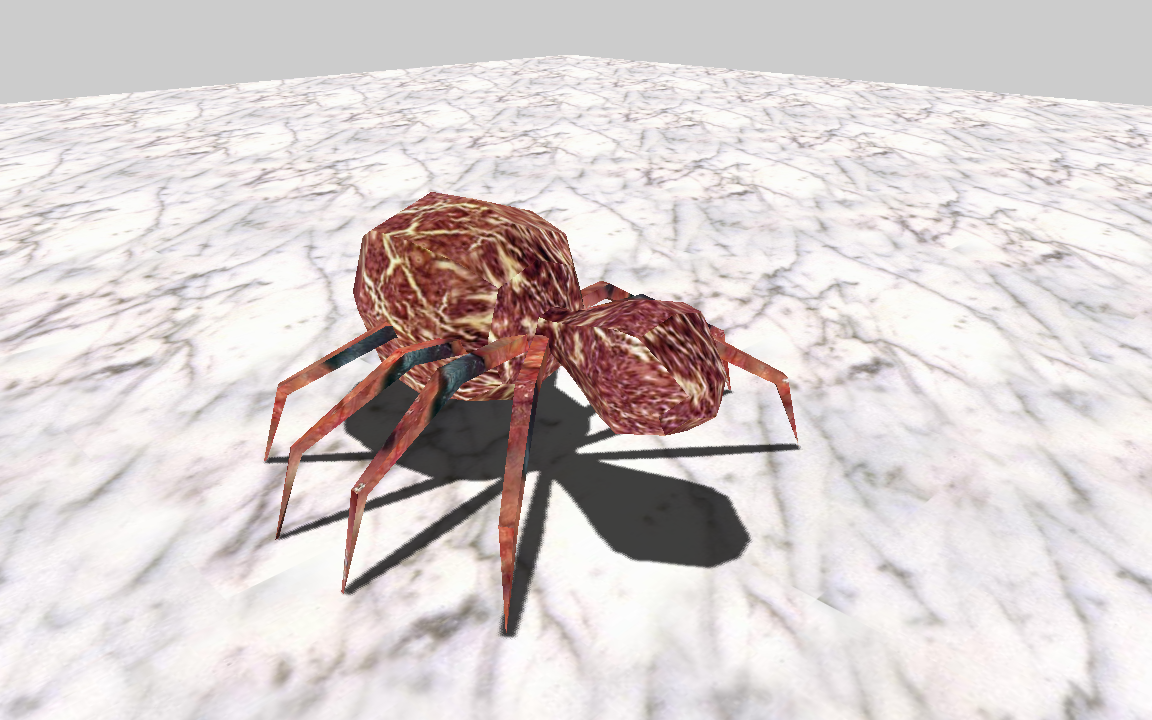
\includegraphics[width=1.8in]{spider_shadow_yes}
%    \caption{Image on the right shows clearly that spider stands on the floor.}
  \end{figure}
\end{frame}

\subsection{Previous Work}
\begin{frame}{Previous Work}
  Both Bitmanagement and Octaga proposed their own shadows extensions.
  We argue that our extensions are a little better :)

  \begin{itemize}
    \item Easier for non-technical authors% (simple \texttt{receiveShadows} field).
    \item Flexible for advanced authors% (shaders, projective mapping).
    \item Nice for implementors% (low-level extensions are easy,
%      and high-level extensions can be transformed to low-level).
  \end{itemize}

  Of course, we would like to see the shadows extensions included
  in the X3D specification.
\end{frame}

\section{Shadow Maps Algorithm}

\begin{frame}{Shadow Maps Algorithm Overview}
  \begin{columns}[T]
    \begin{column}{1.0in}
      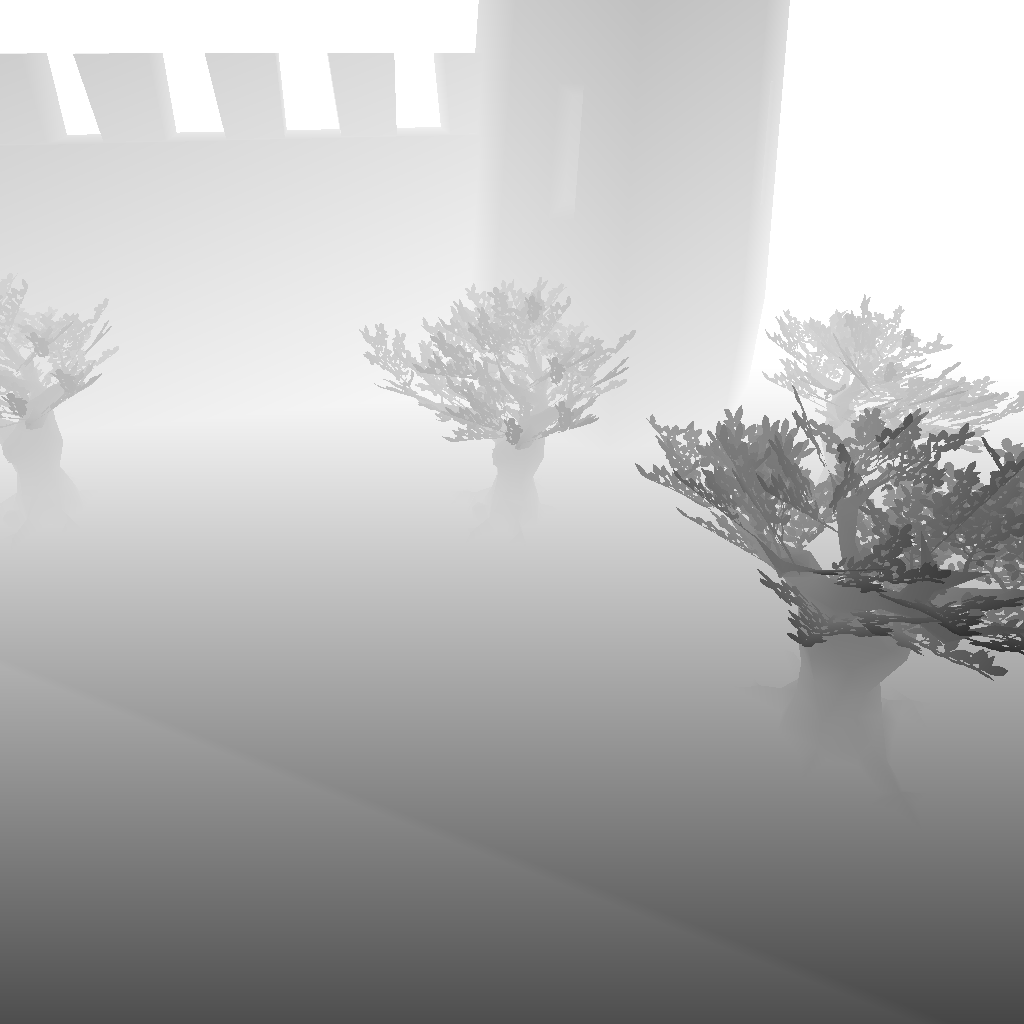
\includegraphics[width=1.2in]{../depths_light_mapped.png}\\
      \vskip10pt
      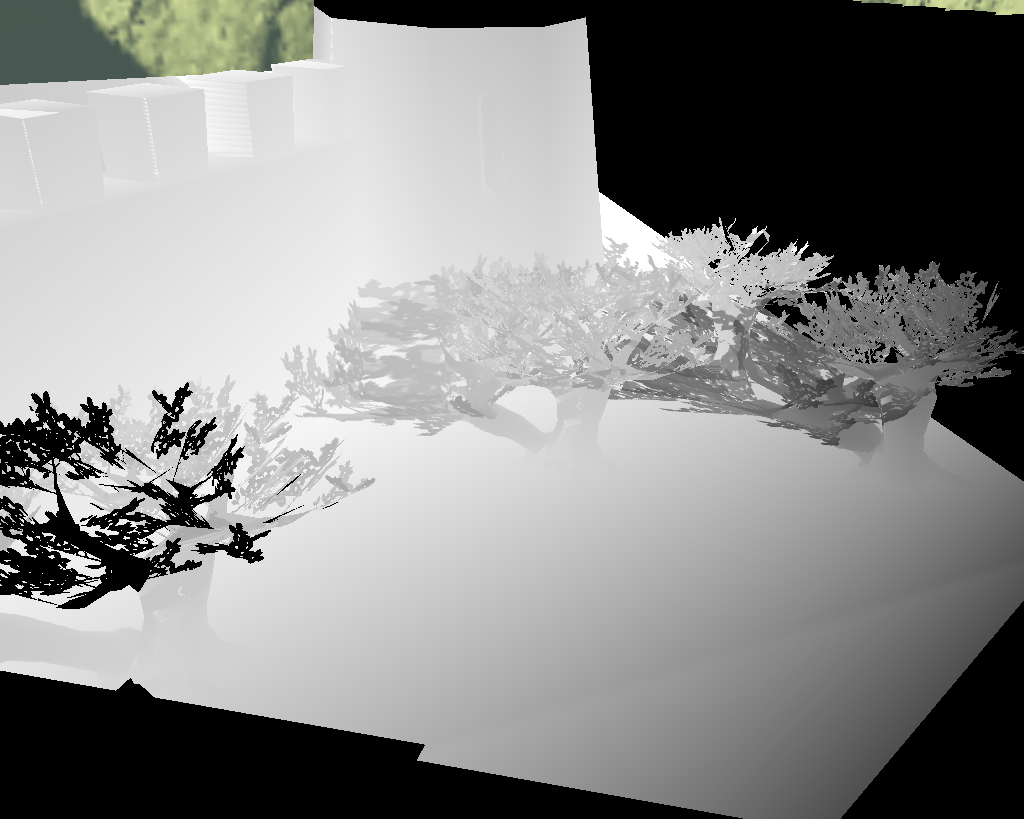
\includegraphics[width=1.2in]{../depths_camera_mapped.png}
    \end{column}
    \begin{column}{3.0in}
      \begin{enumerate}
        \item Render a shadow map from a light source.
      % (needs:
      % - light source parameters
      %   (position, direction, near/far plane etc. --- everything for projection)
      % - texture parameters: size, more later
        \item Project a shadow map when rendering the actual view for the screen.
          This means using a shadow map texture, and calculating a texture
          coordinates such that you know the distance from the light
          at each screen pixel.
      % (needs:
      % - all the light projection parameters from above)
        \item Compare depth value from the shadow map with the actual depth.\\
          \alert{Object in the shadow must be behind an~object obscuring the light.}
      \end{enumerate}
    \end{column}
  \end{columns}
\end{frame}

\begin{frame}{Shadow Maps Terms}
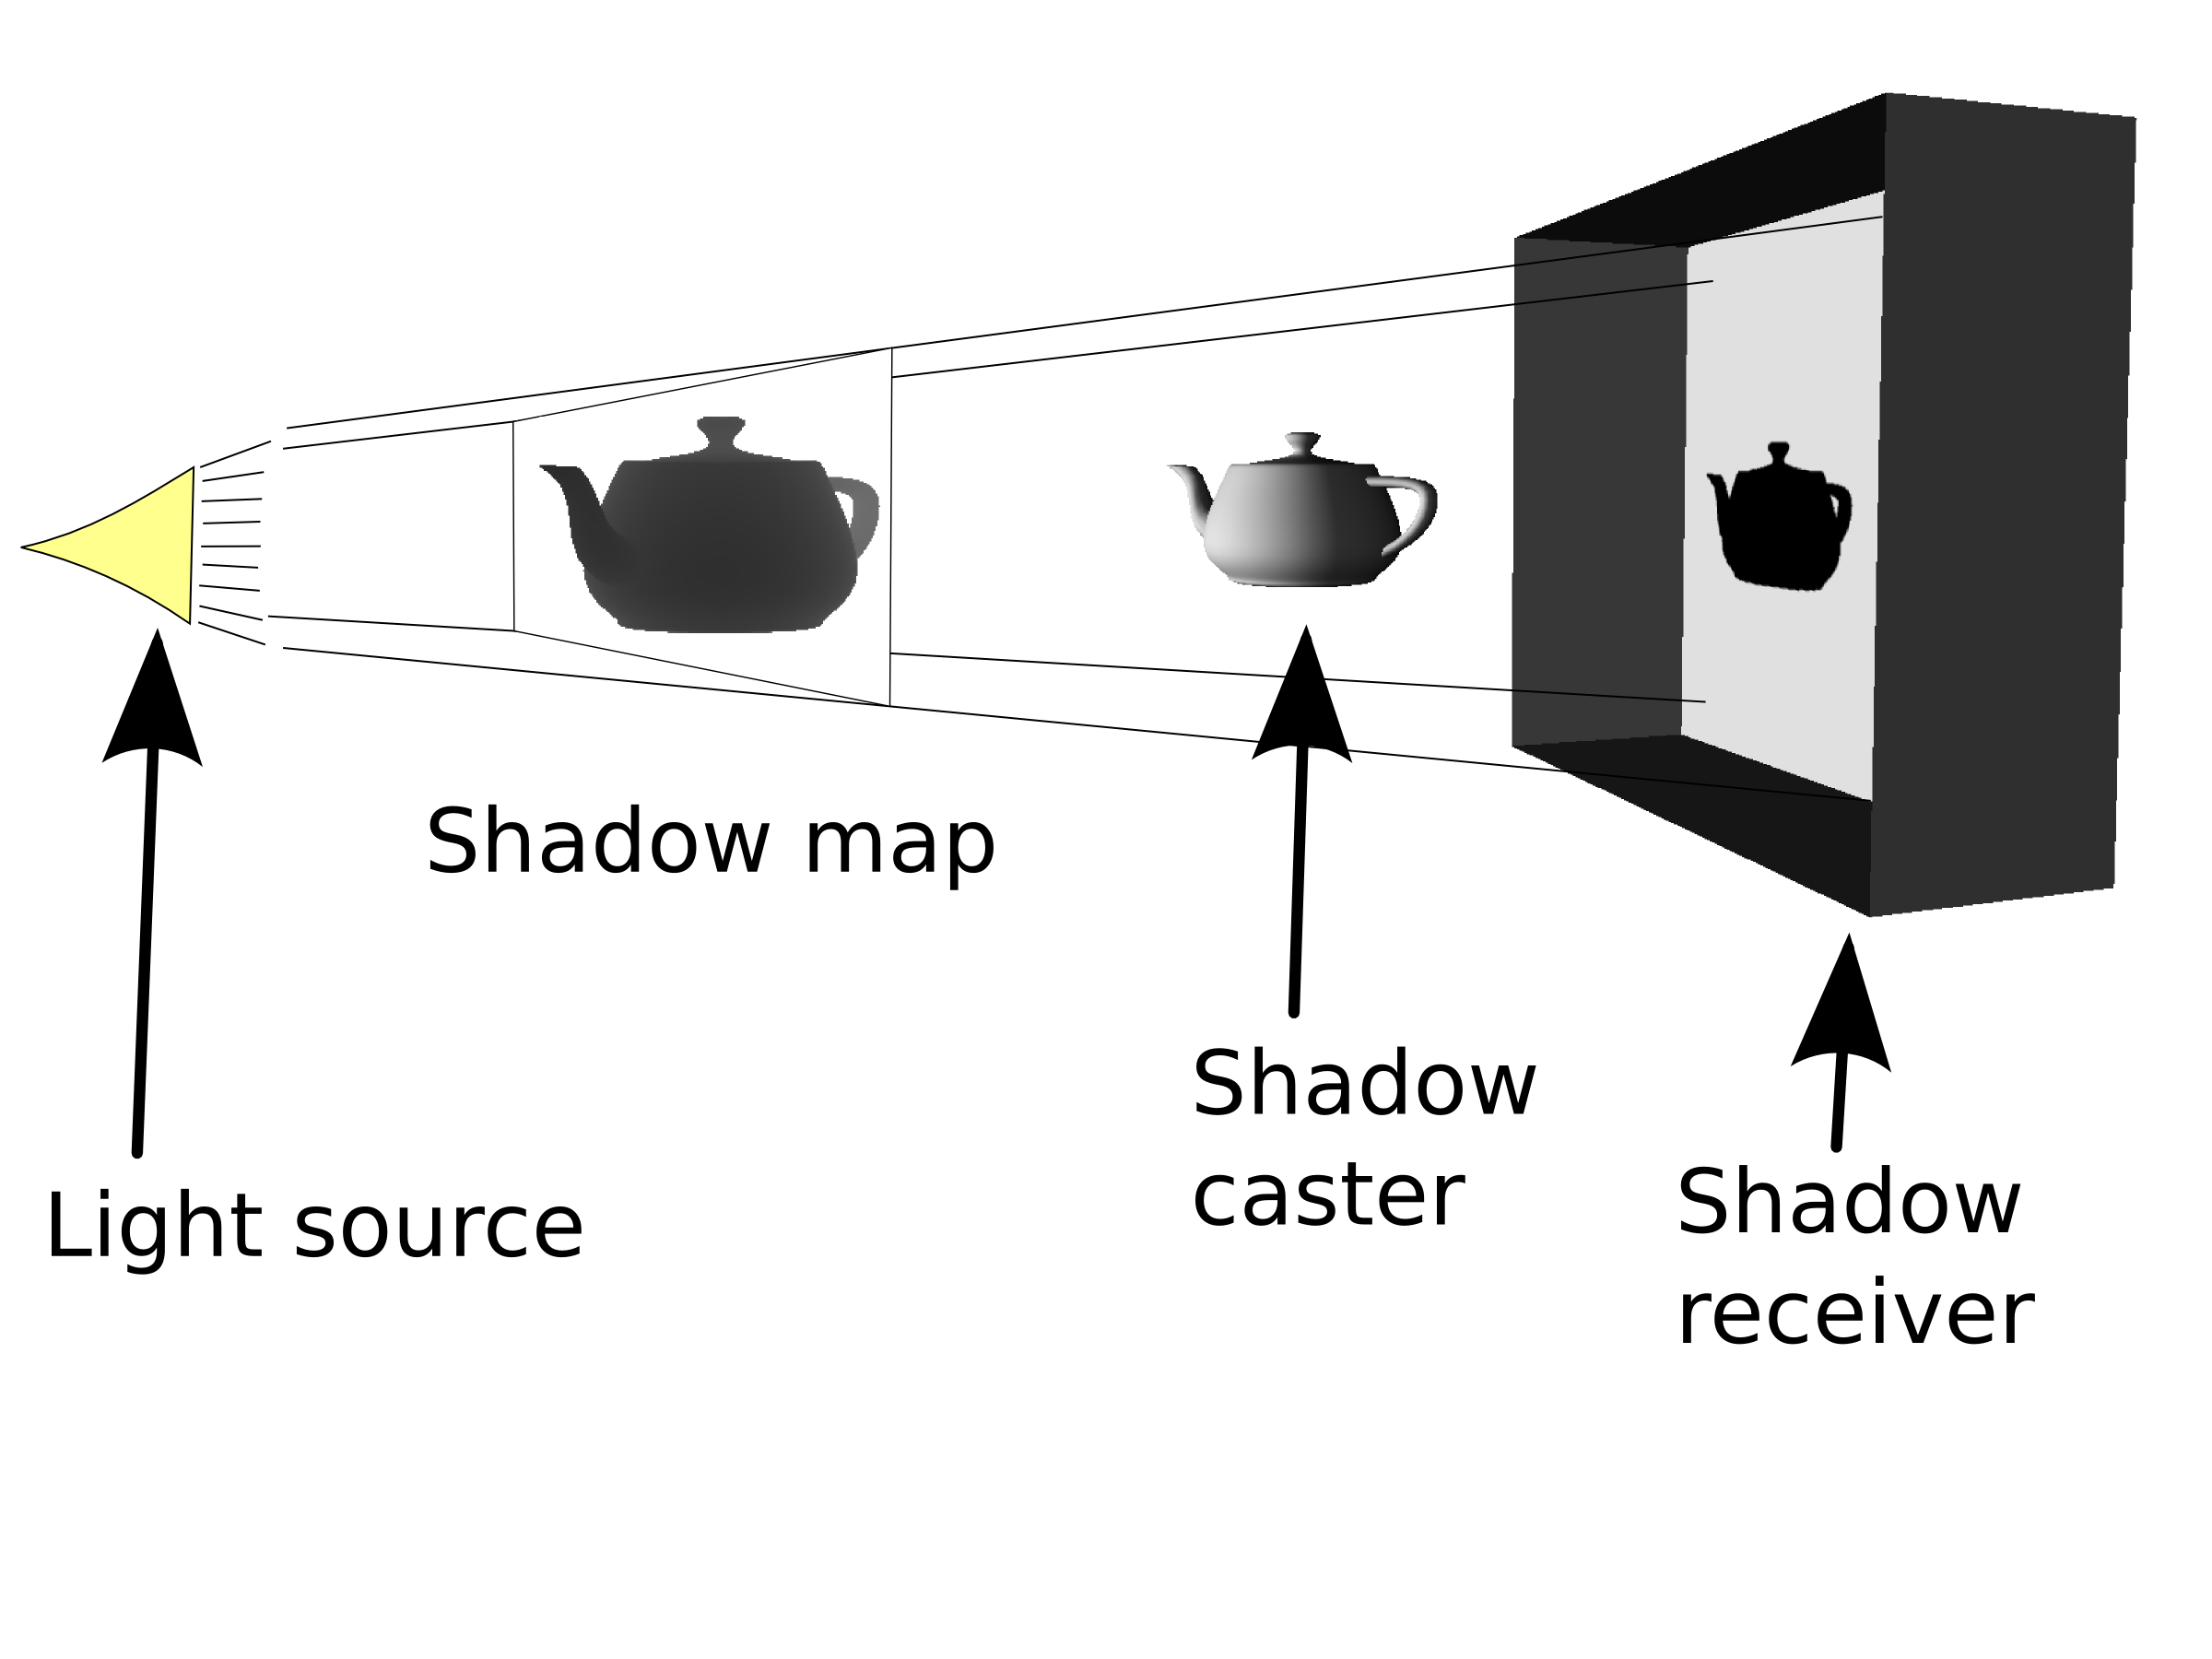
\includegraphics[width=4in]{teapot_final.png}
\end{frame}

\section{High-level Shadows Extensions}

\subsection{Shadow Receivers}

\begin{frame}[fragile]{Define Shadow Receivers}
\begin{block}{New field for the Appearance node}
\begin{semiverbatim}
MFNode  []  \codeem{receiveShadows}  []
  \# [X3DLightNode] list
\end{semiverbatim}
\end{block}

  \begin{itemize}
    \item Very easy to use.\\
      Ideally, the only thing really needed by authors for simplest purposes.
    \item So simple, it's suitable for any shadow algorithm.
    %% \item Can be implemented by transforming the scene to use our
    %%   low-level shadows extensions.
    \item Light contribution (whole, including ambient) is scaled to~zero
      where the light is in the shadow. This way object in~shadow looks
      the same as object outside of light's radius, so things look OK.
  \end{itemize}
\end{frame}

\begin{frame}{Reasoning: Where To Place Shadow Information?}
  \begin{itemize}
    \item \textbf{Separate node}: not natural. We want to make shadows
      commonly used in the scenes, so activating shadows must be easy.
      Also, separate node is not really needed for flexibility.
      %% And not needed, we can get the same level of flexibility with
      %% our receiveShadows and shadowCaster.
    \item \textbf{Casters}:
      there's not much you want to configure on shadow casters.
      You just want to ,,treat everything as shadow caster by default''.
    \item \textbf{Lights}: yes, put some information there, but not flexible enough.
    \item \textbf{Shadow receivers} seem like the best choice:
      \begin{itemize}
        %% \item Not everything needs to receive shadows --- only the most visible,
        %%   bright, large surfaces (floors, walls, main scene objects etc.
    %    \item Flexible.
        \item Natural for authors: shadows change the look of the shadow receiver.
        \item Natural for implementors: shadow receivers must be\\
          rendered in a special way.
      %%   Example (shadow maps with shaders): use a shader that detects are we in shadow by shadow map lookup.
      %%   Example (shadow volumes, all multi-pass approaches): receivers must be drawn many times adding a light contributions.
      \end{itemize}
  \end{itemize}
\end{frame}

\subsection{Shadow Casters}

\begin{frame}[fragile]{Shadow Casters}
  By default, everything casts a shadow.
  Simple global configuration: you can disable casting any shadows
  from this shape.

\begin{block}{New field for the Appearance node}
\begin{semiverbatim}
SFBool  [in,out]  \codeem{shadowCaster}  TRUE
\end{semiverbatim}
\end{block}

  \alert{What if this is too simple?} For complicated cases,
  another field like \texttt{doNotCastShadows} can be added,
  to disable casting shadows for some chosen lights and/or some
  chosen\\ receivers. \alert{In practice, this wasn't needed on our scenes.}
  %% For optimal shadow map rendering, frustum culling etc. takes care of
  %% not rendering everything.
\end{frame}

\subsection{Lights Configuration}

\begin{frame}[fragile]{Shadow Map Parameters}
  In principle, every light by default is capable of casting shadows.
  So you don't \emph{have} to do anything.
  However, you can tweak some shadow maps stuff:

\begin{block}{New field for the X3DLightNode}
\begin{semiverbatim}
SFNode  []  \codeem{defaultShadowMap}  NULL
  \# [GeneratedShadowMap]
\end{semiverbatim}
\end{block}

  The way this works will be clear later, when we describe
  \texttt{GeneratedShadowMap} node. For now, we just note that
  this allows you to:

  \begin{itemize}
    \item manually control when the shadow map is updated,
    \item change shadow map size,
    \item indicate that you want to visualize shadow maps.
  \end{itemize}
\end{frame}

\begin{frame}[fragile]{Lights Projection Parameters}
  For shadow maps, we have to be able to treat lights as cameras.
  So we need some projection parameters.
  When you use \texttt{receiveShadows},
  the browser should be able to calculate suitable values for
  fields below automatically.

  But you can tweak them, for complicated cases and low-level usage.

\begin{block}{New fields for X3DLightNode}
\begin{semiverbatim}
SFFloat  [in,out]  \codeem{projectionNear} 0
SFFloat  [in,out]  \codeem{projectionFar}  0
SFVec3f  [in,out]  \codeem{up} 0 0 0
\end{semiverbatim}
\end{block}

  ...and some additional fields for the \texttt{DirectionalLight}
  and \texttt{SpotLight}, see the paper for details.

%% \begin{block}{New fields for the DirectionalLight node}
%% \begin{semiverbatim}
%% SFVec4f  [in,out]  \codeem{projectionRectangle} 0 0 0 0
%% SFVec3f  [in,out]  \codeem{projectionLocation}  0 0 0
%% \end{semiverbatim}
%% \end{block}

%% \begin{block}{New fields for the SpotLight node}
%% \begin{semiverbatim}
%% SFFloat  [in,out]  \codeem{projectionAngle}  0
%% \end{semiverbatim}
%% \end{block}
\end{frame}

\section{Low-level Shadows Extensions For Shadow Maps}

\subsection{Overview and Examples}

\begin{frame}{Why Low-level Extensions?}
  A couple of cooperating extensions to achieve shadow maps.
  \begin{itemize}
    \item Implementors:
      \begin{itemize}
        \item Very easy to handle in the renderer.
        \item Open a way to handle high-level extensions by transforming to low-level.
      \end{itemize}
    \item Authors:
      \begin{itemize}
        \item \alert{Not easy for authors}: you need to understand how shadow maps work.
        \item But: you can use own shaders (GLSL etc.)
        \item But: you can use projective texturing for other purposes.
      \end{itemize}
  \end{itemize}
\end{frame}

%% \begin{frame}{High-level vs Low-level Extensions}
%%   \begin{block}{High-level extensions}
%%   \begin{itemize}
%%     \item ultra-easy for authors,
%%     \item easy to implement by transforming to low-level extensions.
%%   \end{itemize}
%%   \end{block}

%%   \begin{block}{Low-level extensions}
%%   \begin{itemize}
%%     \item ultra-easy model for implementors,
%%     \item satisfy the advanced authors, that want to write own shaders etc.
%%   \end{itemize}
%%   \end{block}

%%   Having both approaches keeps both the authors and implementors happy.
%% %  And they are connected, so you don't really implement two separate things.
%% \end{frame}

\begin{frame}[fragile]{Example of Low-level Extensions Usage}
\begin{semiverbatim}
DEF MySpot SpotLight \{
  location 0 0 10    direction 0 0 -1
  \codeem{projectionNear 1}    \codeem{projectionFar 20}  \}
Shape \{
  appearance Appearance \{
    texture \codeem{GeneratedShadowMap \{}
      \codeem{light USE MySpot}    \codeem{update "ALWAYS"} \codeem{\}} \}
  geometry IndexedFaceSet \{
    texCoord \codeem{ProjectedTextureCoordinate \{}
      \codeem{projector USE MySpot} \codeem{\}}
    \# ... other IndexedFaceSet fields
  \} \}
\end{semiverbatim}
\end{frame}

\begin{frame}{How Is This Related To High-level Extensions?}
  \alert{The low-level extensions cooperate very nicely with high-level
  extensions described previously:}

  \begin{itemize}
    \item \texttt{receiveShadows} and \texttt{defaultShadowMap}
      may be implemented by transforming the scene to use low-level extensions.

      \textit{How to transform}:
      For each shape with \texttt{receiveShadows}, add to it's textures
      a \texttt{GeneratedShadowMap} node and add to it's tex coords
      a \texttt{ProjectedTextureCoordinate}. Details in the paper.

    \item Rest (light's projection, shadow casters) is simply used as-is.
  \end{itemize}
\end{frame}

\subsection{Generated Shadow Map}

\begin{frame}[fragile]{New X3D Node: Generated Shadow Map}
  You can place this inside e.g. a \texttt{texture} field,
  or as a texture inside shader node (like \texttt{ComposedShader} for GLSL):

\begin{block}{GeneratedShadowMap : X3DTextureNode}
\begin{semiverbatim}
SFString  [in,out]  \codeem{update} "NONE"
  \# ["NONE" | "ALWAYS" | "NEXT\_FRAME\_ONLY"]
SFInt32   []        \codeem{size}  128
SFNode    []        \codeem{light} NULL \# [X3DLightNode]
SFFloat   [in,out]  \codeem{scale} 1.1
SFFloat   [in,out]  \codeem{bias}  4.0
SFString  []        \codeem{compareMode}
  "COMPARE\_R\_LEQUAL" \# ["COMPARE\_R\_LEQUAL"
  \# | "COMPARE\_R\_GEQUAL" | "NONE"]
\end{semiverbatim}
\end{block}
\end{frame}

\subsection{Projected Texture Coordinate}

\begin{frame}[t]{Projecting Textures Explained}

  \vspace{-0.3in}

  \begin{columns}[b]
    \begin{column}{1.6in} \begin{center} Untextured scene \end{center} \end{column}
    \begin{column}{0.1in} \end{column}
    \begin{column}{1.3in} \begin{center} Texture to project \end{center} \end{column}
    \begin{column}{0.1in} \end{column}
    \begin{column}{1.6in} \begin{center} Final scene\\ with projected texture \end{center} \end{column}
  \end{columns}
  \begin{columns}[c]
    \begin{column}{1.6in}
      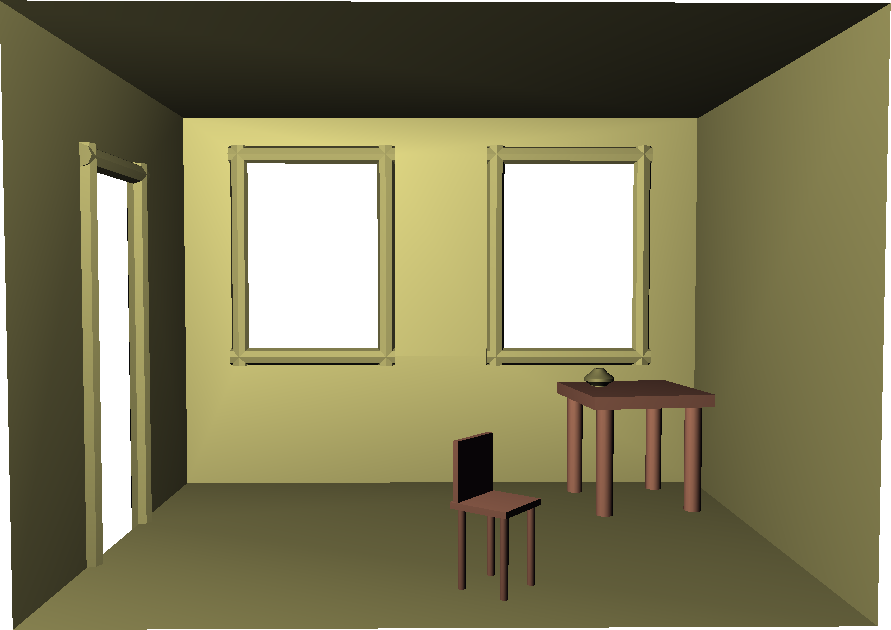
\includegraphics[width=1.6in]{projector_room_no}
    \end{column}
    \begin{column}{0.1in}
      \Large{\textbf{+}}
    \end{column}
    \begin{column}{1.3in}
      \includegraphics[width=1.2in]{test_texture}
    \end{column}
    \begin{column}{0.1in}
      \Large{\textbf{=}}
    \end{column}
    \begin{column}{1.6in}
      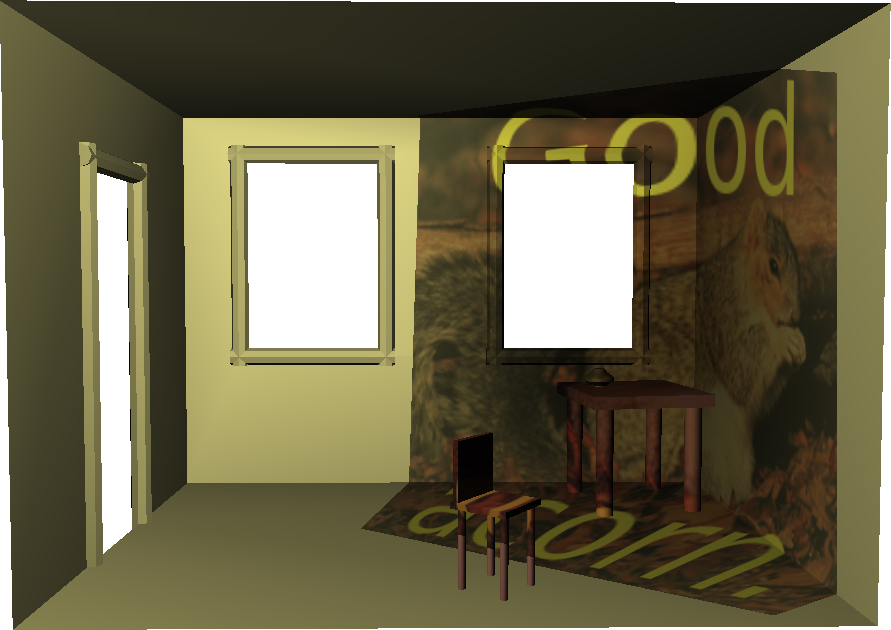
\includegraphics[width=1.6in]{projector_room_yes}
    \end{column}
  \end{columns}

  \vspace{0.15in}

  \begin{columns}[c]
    \begin{column}{1in}
      Final scene,\\
      as seen from\\
      the projector:\\
    \end{column}
    \begin{column}{1.7in}
      \hspace{-0.75in}
      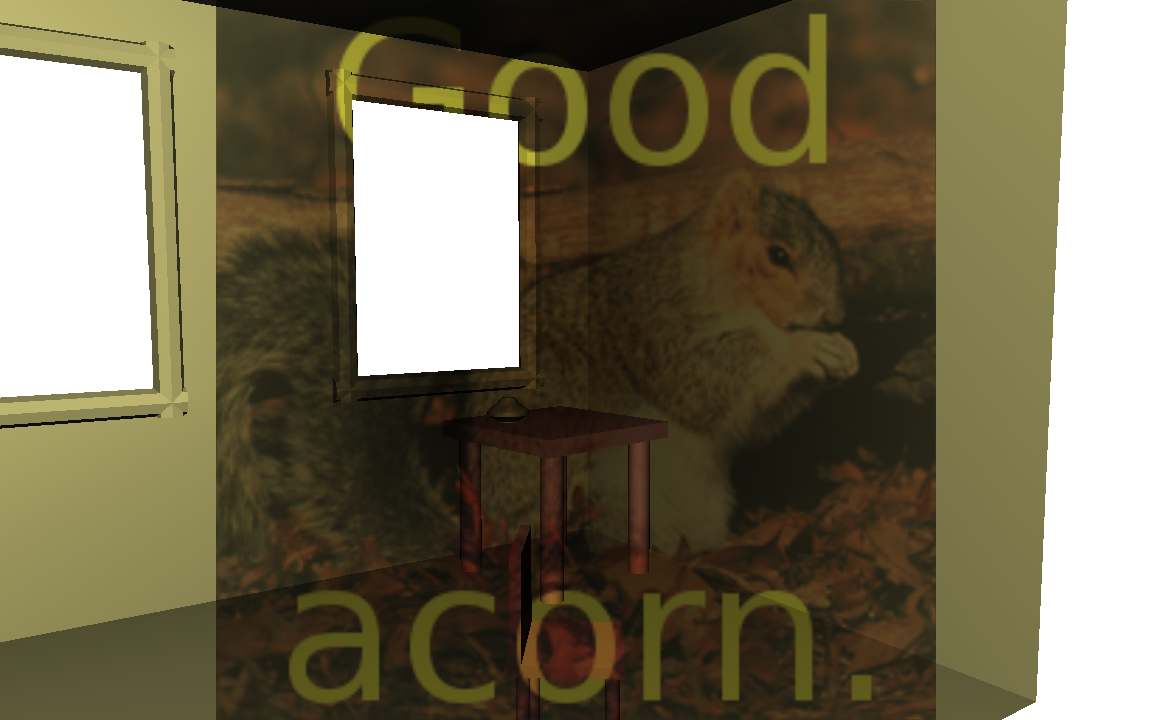
\includegraphics[width=1.6in]{projector_room_projector_view}
    \end{column}
  \end{columns}

\end{frame}

\begin{frame}[fragile]{New X3D Node: Projected Texture Coordinate}
  You can place this inside e.g. \texttt{texCoord} fields:

\begin{block}{ProjectedTextureCoordinate : X3DTextureCoordinateNode}
\begin{semiverbatim}
SFNode  [in,out]  \codeem{projector}  NULL
  \# [SpotLight, DirectionalLight,
  \# X3DViewpointNode]
\end{semiverbatim}
\end{block}

  %% \begin{columns}[T]
  %%   \begin{column}{1in}
  %%     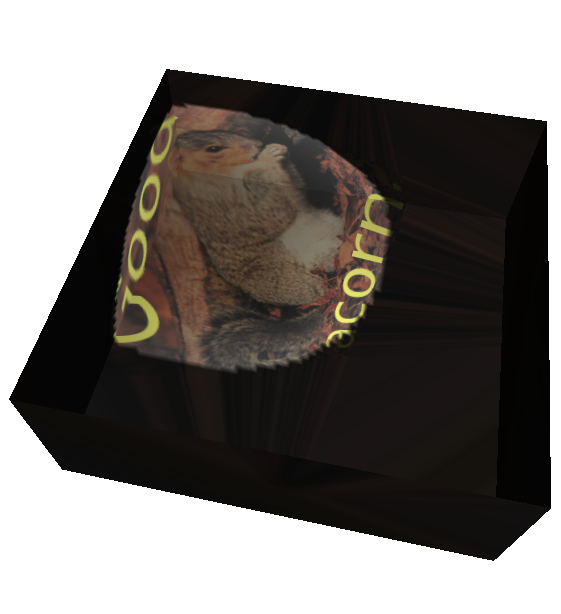
\includegraphics[width=1.2in]{../tex_projected_spot_1.png}
  %%   \end{column}
  %%   \begin{column}{3in}
      Generates texture coordinates that project (cast) a texture.
      \begin{itemize}
        \item For shadow maps: project your shadow map from a light source.
        \item You can also project a normal texture (e.g. color \texttt{MovieTexture}).
        \item You can also project from a viewpoint (e.g. to cast a headlight texture).
      \end{itemize}
  %%   \end{column}
  %% \end{columns}
\end{frame}

%% \begin{frame}{How the High-level Extensions Map To Low-level}
%%   The \texttt{receiveShadows} field may be implemented by transforming
%%   X3D graph to low-level nodes:

%%   \begin{itemize}
%%     \item Create new \texttt{GeneratedShadowMap} node, or use
%%       an existing \texttt{defaultShadowMap} of the light source.
%%     \item Add this \texttt{GeneratedShadowMap} node
%%       to the appearance \texttt{texture}. You may need to change
%%       the existing texture to the \texttt{MultiTexture} node, to preserve the old
%%       texture.
%%     \item Create appropriate \texttt{ProjectedTextureCoordinate} node and add
%%       it to the geometry \texttt{texCoord} field. You may need to change
%%       the texture coordinate to the \texttt{MultiTextureCoordinate} node,
%%       to preserve the old texture coordinates.
%%     \item If you use shaders, then add appropriate shader nodes,
%%       and add your \texttt{GeneratedShadowMap} node to them too.
%%   \end{itemize}
%% \end{frame}

\section{Summary}
% Keep the summary *very short*.

\begin{frame}{Summary}

\begin{block}{High-level extensions to easily get shadows}
  \begin{itemize}
    \item Define shadow receivers by the \texttt{receiveShadows} field.
%    \item Optionally place GeneratedShadowMap inside ,,defaultShadowMap''.
    \item Easy to use, easy to implement basing on low-level extensions.
  \end{itemize}
\end{block}

\begin{block}{Low-level extensions to fully control shadow maps}
  \begin{itemize}
    \item Define shadow receivers by explicitly adding
      \texttt{GeneratedShadowMap} and \texttt{ProjectedTextureCoordinate}
      to textures and tex coords.
    \item Easy to implement.
    \item Projective texturing available also independently.
    \item Usable with custom shaders.
  \end{itemize}
\end{block}

% - Cooperating nicely: shadow caster, light's projection parameters
% are the same. GeneratedShadowMap used inside defautShadowMap
% may be simply copied into shape's ,,texture'' during transformation.

% Implementation:
% - Done :)
%   Also Variance Shadow Maps implemented (no change to extensions needed).
% - We also have shadow volumes and ray-tracer, that currently honor shadow caster field but not yet receiveShadows. But will be...
\end{frame}

\begin{frame}[t]

\begin{center}
{\Large Thank you for your attention!}
\end{center}

\vspace{0.25in}

\begin{center}
{\Huge \alert{Questions?}}
\end{center}

\vspace{0.25in}

\begin{center}
{\Large Visit our VRML engine on
{\color{blue} \textbf{\texttt{http://vrmlengine.sourceforge.net/}}}}
\end{center}
\end{frame}

\end{document}
